\documentclass[a4paper, 11pt, UTF8]{ctexart}
\usepackage{graphicx}
\usepackage{geometry}
\usepackage{enumerate}
\usepackage{caption}
\usepackage{subfigure}
\usepackage{float}
\usepackage{hyperref}

\hypersetup{hidelinks}


\title{基本功能测试方案}

\author{机械108 \qquad 张益铭 \qquad 2021010552}

\date{\today}

\geometry{left=3cm, right=3cm, top=4cm, bottom=4cm}

\begin{document}

\maketitle

\tableofcontents

\rightline{p.s. 点击目录进行跳转 :)}

\newpage

\section{正常输入}

测试程序加、减、乘、取余计算情况。

输入1:129785 * 1263 + 21738 * 3124 + 231245 * 412 \% 135 * 123 + 112 - 12 + 156 * 89

输出1:231849946

\begin{figure}[H]
    \centering
    \caption{四则运算}
    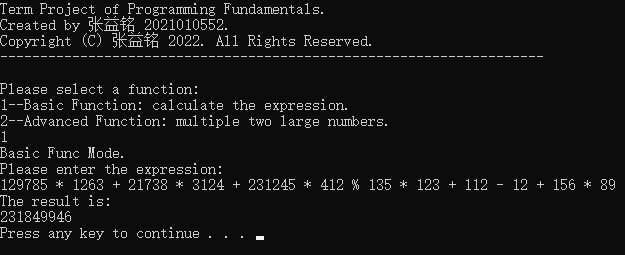
\includegraphics[width=0.8\textwidth]{t1.png}    
\end{figure}

输入2:0 + 1 - 2 * 3 \% 4 + 5 - \dots\dots + 497 - 498 * 499 \% 500

输出2:30875

\begin{figure}[H]
    \centering
    \caption{较长数据测试}
    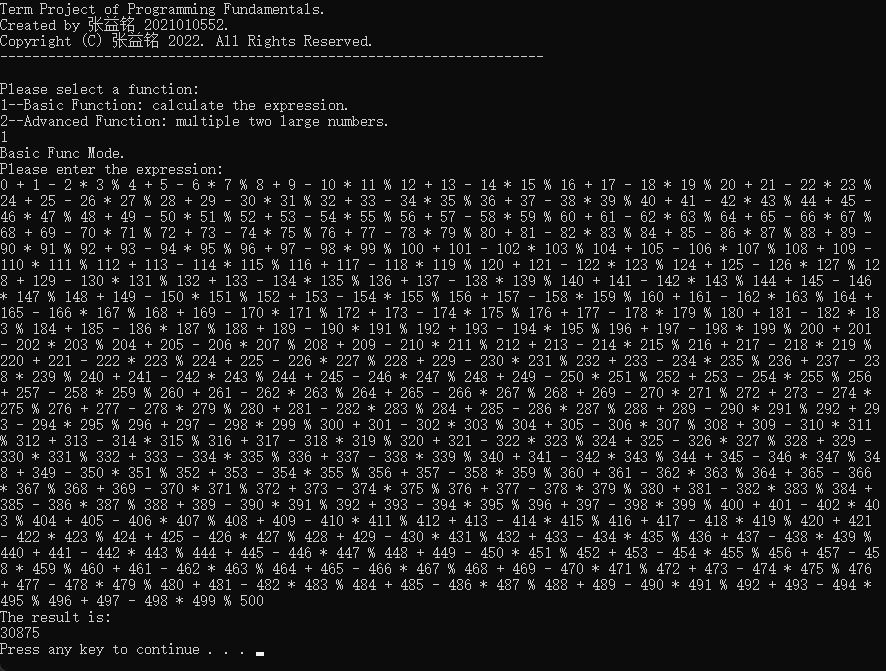
\includegraphics[width=0.8\textwidth]{t2.png}    
\end{figure}

\section{鲁棒性测试}

\subsection{选择功能}

输入3:abcd

输出3:Invalid function type!

\begin{figure}[H]
    \centering
    \caption{输入非数字}
    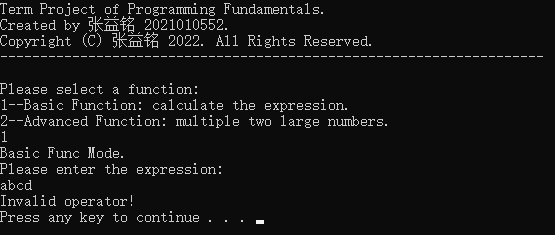
\includegraphics[width=0.8\textwidth]{t3.png}    
\end{figure}

输入4:0

输出4:Invalid function type!

\begin{figure}[H]
    \centering
    \caption{输入1、2之外的数}
    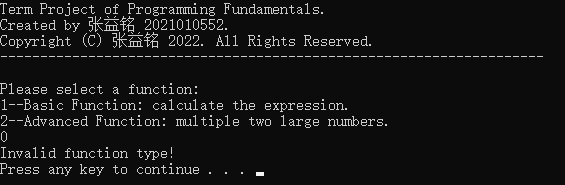
\includegraphics[width=0.8\textwidth]{t4.png}
\end{figure}

\subsection{输入表达式}

输入5:

输出5:Please enter the expression!

\begin{figure}[H]
    \centering
    \caption{不输入}
    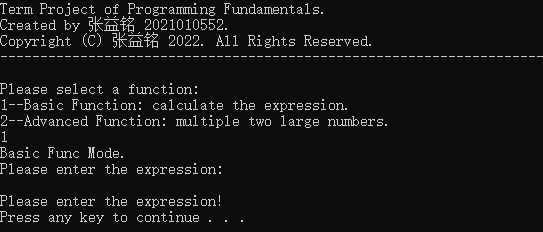
\includegraphics[width=0.8\textwidth]{t5.png}
\end{figure}

输入6:*15+1

输出6:Operator missing operand!

\begin{figure}[H]
    \centering
    \caption{第一位不是数字}
    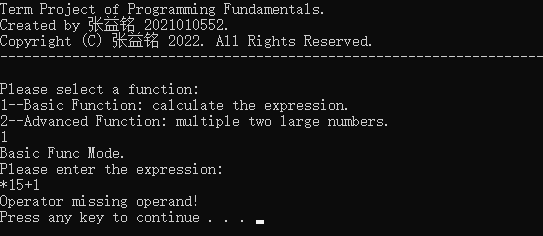
\includegraphics[width=0.8\textwidth]{t6.png}    
\end{figure}

输入7:1 + (-2)*3

输出7:Please enter expressions in English!

\begin{figure}[H]
    \centering
    \caption{输入中文括号}
    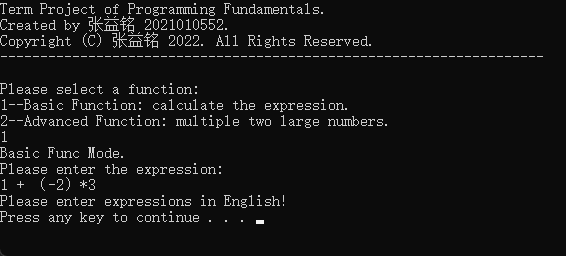
\includegraphics[width=0.8\textwidth]{t7.png}    
\end{figure}

输入8:abcd

输出8:Invalid operator!

\begin{figure}[H]
    \centering
    \caption{输入不是数字}
    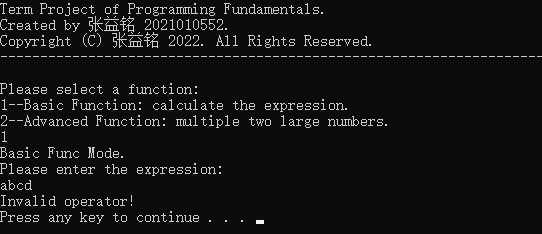
\includegraphics[width=0.8\textwidth]{t8.png}    
\end{figure}

输入9:1 + 2 * + 3

输出9:Operator missing operand!

\begin{figure}[H]
    \centering
    \caption{缺少运算符/数字}
    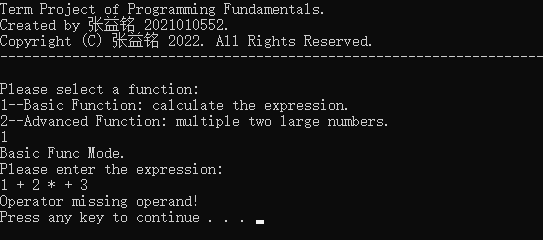
\includegraphics[width=0.8\textwidth]{t10.png}    
\end{figure}

输入10:156 * ((-1) * 13

输出10:Parenthesis DO NOT match!

\begin{figure}[H]
    \centering
    \caption{括号不匹配}
    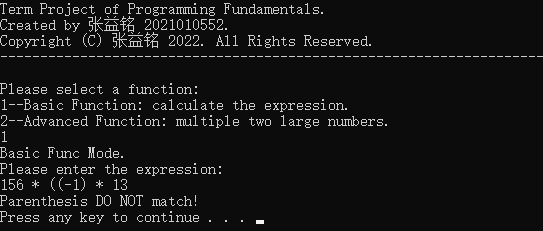
\includegraphics[width=0.8\textwidth]{t9.png}
\end{figure}

输入11:12 \% (2-2)

输出11:Modulo 0!

\begin{figure}[H]
    \centering
    \caption{对0取余}
    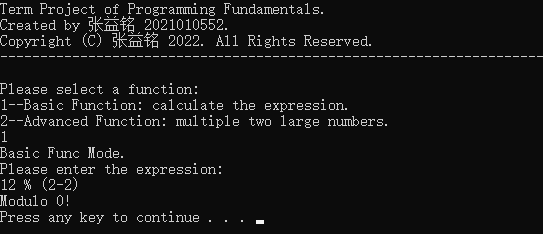
\includegraphics[width=0.8\textwidth]{t11.png}
\end{figure}

输入12:123+456*

输出12:Operator missing operand!

\begin{figure}[H]
    \centering
    \caption{最后一位是运算符}
    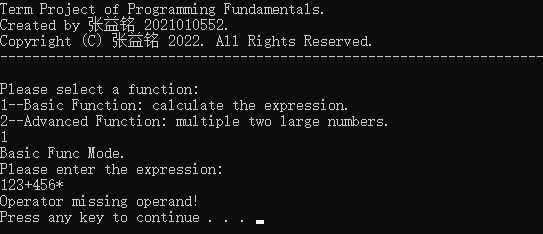
\includegraphics[width=0.8\textwidth]{t12.png}
\end{figure}

输入13:12345678901

输出13:Number out of range!

\begin{figure}[H]
    \centering
    \caption{数字过长}
    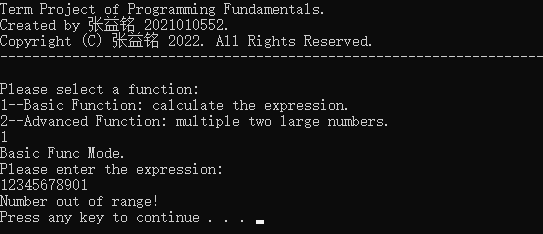
\includegraphics[width=0.8\textwidth]{t13.png}
\end{figure}

\end{document}